\documentclass[]{article}
\usepackage{lmodern}
\usepackage{amssymb,amsmath}
\usepackage{ifxetex,ifluatex}
\usepackage{fixltx2e} % provides \textsubscript
\ifnum 0\ifxetex 1\fi\ifluatex 1\fi=0 % if pdftex
  \usepackage[T1]{fontenc}
  \usepackage[utf8]{inputenc}
\else % if luatex or xelatex
  \ifxetex
    \usepackage{mathspec}
  \else
    \usepackage{fontspec}
  \fi
  \defaultfontfeatures{Ligatures=TeX,Scale=MatchLowercase}
\fi
% use upquote if available, for straight quotes in verbatim environments
\IfFileExists{upquote.sty}{\usepackage{upquote}}{}
% use microtype if available
\IfFileExists{microtype.sty}{%
\usepackage{microtype}
\UseMicrotypeSet[protrusion]{basicmath} % disable protrusion for tt fonts
}{}
\usepackage[margin=1in]{geometry}
\usepackage{hyperref}
\hypersetup{unicode=true,
            pdftitle={Comparing the precision of different estimates},
            pdfauthor={Peder M. Isager},
            pdfborder={0 0 0},
            breaklinks=true}
\urlstyle{same}  % don't use monospace font for urls
\usepackage{longtable,booktabs}
\usepackage{graphicx,grffile}
\makeatletter
\def\maxwidth{\ifdim\Gin@nat@width>\linewidth\linewidth\else\Gin@nat@width\fi}
\def\maxheight{\ifdim\Gin@nat@height>\textheight\textheight\else\Gin@nat@height\fi}
\makeatother
% Scale images if necessary, so that they will not overflow the page
% margins by default, and it is still possible to overwrite the defaults
% using explicit options in \includegraphics[width, height, ...]{}
\setkeys{Gin}{width=\maxwidth,height=\maxheight,keepaspectratio}
\IfFileExists{parskip.sty}{%
\usepackage{parskip}
}{% else
\setlength{\parindent}{0pt}
\setlength{\parskip}{6pt plus 2pt minus 1pt}
}
\setlength{\emergencystretch}{3em}  % prevent overfull lines
\providecommand{\tightlist}{%
  \setlength{\itemsep}{0pt}\setlength{\parskip}{0pt}}
\setcounter{secnumdepth}{0}
% Redefines (sub)paragraphs to behave more like sections
\ifx\paragraph\undefined\else
\let\oldparagraph\paragraph
\renewcommand{\paragraph}[1]{\oldparagraph{#1}\mbox{}}
\fi
\ifx\subparagraph\undefined\else
\let\oldsubparagraph\subparagraph
\renewcommand{\subparagraph}[1]{\oldsubparagraph{#1}\mbox{}}
\fi

%%% Use protect on footnotes to avoid problems with footnotes in titles
\let\rmarkdownfootnote\footnote%
\def\footnote{\protect\rmarkdownfootnote}

%%% Change title format to be more compact
\usepackage{titling}

% Create subtitle command for use in maketitle
\providecommand{\subtitle}[1]{
  \posttitle{
    \begin{center}\large#1\end{center}
    }
}

\setlength{\droptitle}{-2em}

  \title{Comparing the precision of different estimates}
    \pretitle{\vspace{\droptitle}\centering\huge}
  \posttitle{\par}
    \author{Peder M. Isager}
    \preauthor{\centering\large\emph}
  \postauthor{\par}
      \predate{\centering\large\emph}
  \postdate{\par}
    \date{2019-04-12}


\begin{document}
\maketitle

\hypertarget{abstract}{%
\section{Abstract}\label{abstract}}

Given that we define replication value conceptually as a ratio of
``impact'' over ``corroboration'', and given that we want to derive
quantifiable metrics from this definition, we need to give a reasonable
and quantitative operationalization of corroboration. Here, I first
propose to approximate corroboration through the more narrow concept
``precision of the estimate''. I then quantify precision of the estimate
as the variance of Fisher's \emph{Z}, which only depends on sample size
(although the variance of the common language effect size \emph{A} could
also be used for group comparisons, if information about group sample
sizes is available).

\begin{figure}
\centering
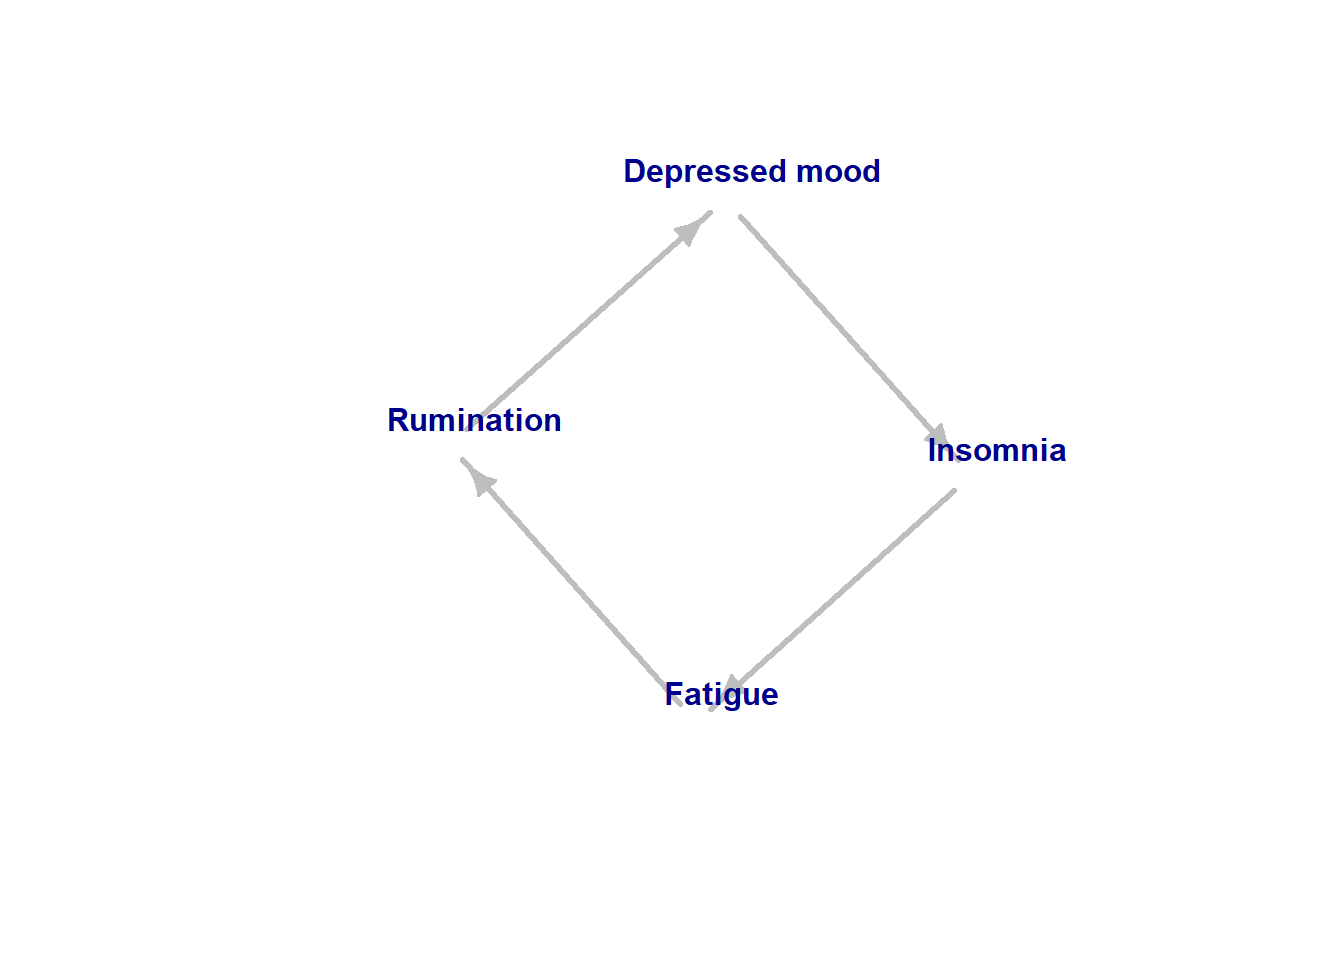
\includegraphics{2019-04-12-quantifying-and-comparing-the-precision-of-multiple-estimates_files/figure-latex/figs-1.pdf}
\caption{\label{fig:figs}plotting example}
\end{figure}

\hypertarget{looking-for-needles-in-haystacks-of-findings}{%
\section{Looking for needles in haystacks of
findings}\label{looking-for-needles-in-haystacks-of-findings}}

When we seek to replicate findings in psychology, we often face the
problem that there are multiple findings we could replicate, of which we
will only have resources available to address one or a few. This means
that we will have to decide which finding would be the most valuable to
spend our time replicating. But the process of study selection can
itself be a challenge. For example, in a replication effort I am
currently involved with, we have more than 1000 studies we could
consider for replication, each of which will contain multiple findings.
We would like to discover and choose from the most valuable findins to
replicate in this sample, but we simply do not have the time or
cognitive capacity available to manually inspect and compare 1000
studies to each other. Is there a way to evaluate this set of studies
and identify the most promising replication candidates, without
committing years of our time to manual inspection?

\hypertarget{quantifying-replication-value}{%
\section{Quantifying replication
value}\label{quantifying-replication-value}}

Together with members of the Open Science collaboration I am currently
trying to develop a approach for quantifying the ``replication value''
of published findings through formulas. Quantified estimates of
replication value can be calculated relatively quickly, which should
allow researchers to evaluate large sets of findings and identify
promising replication candidates. Manual inspection will still be
required, but can be focused on the most promising candidates from the
formula evaluation. As such, the aim is increase the efficiency of
manual inspection efforts, and to increase the chance that high-value
replication targets are discovered. We propose that the replication
value of a finding can be conceptually thought of as a combination of
the impact and the corroboration of that finding in the literature:

\[
\begin{equation}
RV=\frac{Impact}{Corroboration}
\label{eq:repval}
\tag{1}
\end{equation}
\]

In words, the more impactful a study has become, the higher its
replication value (``RV'' in formula) will be. Conversely, the better
corroborated a finding has become, the lower its replication value will
be. We can gain an understanding of what researchers might take as
indicators of ``impact'' and ``corroboration'' by surveying the
literature of published replication studies. In
\href{https://pedermisager.netlify.com/post/what-to-replicate/}{a
previous blog post} I have attempted to provide a brief summary.

There are multiple issues and caveats that will need to be considered
when trying to approximate the ``true'' replication value of a finding
through quantitative information. Among other things, we need to know
whether formula \(\eqref{eq:repval}\) captures our conceptual
understanding of replication value, whether it can be expressed in
quantitative terms, and if so, how to operationalize the concepts in
contained in formula \(\eqref{eq:repval}\) numerically. In this post I
will deal with one rather fundamental question: \textbf{How do we
quantify corroboration?}

\hypertarget{quantifying-corroboration}{%
\section{Quantifying corroboration}\label{quantifying-corroboration}}

There are many aspects of corroboration that we could consider for the
purpose of calculating replication value, each of which would
subsequently inform the quantitative information of interest to us
(Lakens 2019). For example, we might want to prioritize findings for
publication that have low evidence in favor of certain hypotheses
compared to others (Field et al. 2018). Or we may want to prioritize
findings that display signs of biased and/or erroneous reporting (Brown
and Heathers 2017; Heathers et al. 2018; Simonsohn, Nelson, and Simmons
2014; Dwan et al. 2008; Nuijten et al. 2017; Kerr 1998). Or perhaps we
simply want to replicate findings where we are surprised about the
likelihood of the data under the null hypothesis.

Here I choose to focus on precision. Precision of the estimate can
normally be thought of as the variance, standard error, or
confidence/credible interval of a measurement (Borenstein, chapter 8).
However, precision can also be related to qualitative estimates
(e.g.~people generally experience set S of side effects after taking
drug D) and predictions involving multiple estimates (e.g.~people
experience side effect X, Y, and Z, with magnitude A, B and C,
respectively, after taking drug D). More generally, precision can be
thought of as the reciprocal to uncertainty. That is, for any estimand
(a set, a magnitude, a mean, etc.), the less uncertain we are about
whether it could be this way or that, the more precisely it is
estimated. Precision can be considered one subcategory of what
determines the corroboration of a finding. Everything else being equal,
we may assume that a finding that has been estimated precisely has
attained more corroboration than a finding that has been estimated
imprecisely. Consequently, we may also assume that, everything else
being equal, a precisely measured estimate is less replication-worthy
than an imprecisely measured estimate, which is what follows from our
conceptual definition of replication value in formula
\(\eqref{eq:repval}\).

Of course, everything else is usually not equal, and corroboration as a
construct encompasses much more than the precision of an estimate. This
is partly why manual inspection should always be part of evaluating
whether one finding is truly more worth replicating than another. Still,
we consider it plausible that precision of the estimate is positively
correlated with latent corroboration on average. By substituting
precision for corroboration in the replication value formula
\(\eqref{eq:repval}\), we will essentially prioritize findings for
replication that have been imprecisely measured in the literature thus
far.

When comparing the precision of a set of estimates, we may want to
compare two or more effects that stem from different designs, and that
are expressed on different scales. That is, sometimes we may wish to
compare effects expressed in Cohen's \emph{d} to effects expressed in
Pearson's \emph{r}, odds ratio, etc. In order to compare effects
expressed on different scales, we need an estimate of precision that is
comparable across the scales. Otherwise, we cannot meaningfully compare
the corroboration of two different kinds of effects. Consider a
confidence interval \emph{CI}{[}2.27, 14.04{]} for an effect expressed
in units of Cohen's \emph{d}. In the context of most behavioral
research, this would be considered a highly imprecise measurement. Now
consider a confidence interval \emph{CI}{[}0.75, 0.99{]} expressed in
units of Pearson's \emph{r}. If directly compared, the latter interval
might appear more precise than the former, but this is simply due to the
fact that Pearson's \emph{r} is a non-linear scale bounded between -1
and 1, whereas Cohen's \emph{d} is a linear scale bounded between -∞ and
∞. In fact, the two intervals in this example are the same interval,
expressed in two units of measurement. We can compare their precision
only if we first convert either interval into the scale of the other, or
convert both intervals into some other common unit of measurement. It is
not meaningful to compare intervals measured on different scales
directly.

This problem is similar to that faced by meta-analysts who want to
compare effect sizes measured on different scales (Borenstein 2009,
Chapter 7). However, the two problems are not quite the same. For
example, meta-analyses ideally deal with studies on the same effect that
are either ``close'' replications (LeBel et al. 2018), or at least
conceptually similar. The replication value, on the other hand, should
be comparable even for studies that are not on the same topic. In
addition, the effect size is often the statistic of interest in
traditional meta-analysis. In contrast, since the size of the effect is
orthogonal to the precision of the estimate of the effect, effect size
should be irrelevant for our corroboration estimate.

The rest of this discussion will be consentrated on finding a suitable
operationalization of ``precision''. However, before venturing on,
readers should keep in mind that the aspect of corroboration we choose
to focus on will shape the entire rationale for any quantifiable
operationalization of corroboration. The following discussion is based
on the assumption that precision is the aspect of corroboration that we
would like to operationalize. If instead we would like to focus on other
aspects of corroboration (e.g.~Field et al. 2018), the arguments that
follow will not necessarily hold, and some operationalizations that are
considered inappropriate in the context of precision may very well be
relevant for approximating other aspects of corroboration (and vice
versa).

\hypertarget{requirements-for-a-precision-statistic}{%
\subsection{Requirements for a precision
statistic}\label{requirements-for-a-precision-statistic}}

In order for a precision statistic to be useful in the context of the
replication value, we should expect it to adhere to the following
requirements:

\begin{itemize}
\item
  \textbf{Standardization:} The measure must express precision on a
  standardized scale. If calculated for a number of estimates, the
  precision of the estimates must always be comparable/on the same
  scale.
\item
  \textbf{Meta-analytic updating:} we must be able to update the
  precision statistic after a replication is performed. Replication
  generally adds information about a finding, and should tend to
  increase the precision of an estimate and thus decrease the
  replication value of a finding.
\item
  \textbf{Size independence:} The measure must not depend on the size of
  the effect.
\item
  \textbf{Exhaustiveness:} The measure must accurately represent the
  precision of the estimate. Therefore, the measure should take all
  relevant aspects of the precision into account when they are
  available, such as the standard deviation of the estimate, the sample
  size, the between-condition correlation for repeated measures, etc.
\end{itemize}

Each requirement is supported by a specific rationale related to the
desired functions of the replication value. If the standardization
requirement is violated, it becomes impossible to know if differences
between effects are due to differences in impact and precision, or if
the compared effects are equally precise but measured on different
scales. If the meta-analytic updating requirement is violated, there is
no mechanism for updating the precision estimate after replications are
conducted. This would disrupt a central feature of the replication
value; after a finding is replicated, its replication value should
decrease. If the effect-size independence requirement is violated, the
replication value will become biased (either favorably or unfavorably)
towards findings with a large effect size. This is undesirable if we
assume that the goal of replication is to reduce uncertainty in an
estimate regardless of whether the true effect is large, small or zero
(we may not always want to assume this of course). If the exhaustiveness
requirement is violated, we risk misrepresenting the actual precision of
certain measures. For example, two estimates may have the same sample
size and yet, if standard deviations or within-subject correlation
differs substantially between the estimates, one estimate can be much
more precise than the other. The exhaustiveness requirement could be
considered less critical than the other three however. As long as the
error introduced by violating it is random, the precision estimate
becomes less accurate by not accounting for all relevant factors, but
not categorically invalid. It still tracks our conceptual understanding
of ``precision'' to some degree. However, more serious issues arise when
not accounting for relevant information leads to systematic bias. For
example, if we ignore inter-trial correlation and the fact that each
subject contributes at least two data points in within-subject designs,
the precision of the estimate (and hence, the replication value) of
within-subject measurements will be overestimated compared to
between-subjects measurements. In this case, not accounting for the
difference in design would ultimately lead us to violate the
standardization requirement.

\hypertarget{candidate-statistics}{%
\subsection{Candidate statistics}\label{candidate-statistics}}

There are several potential candidate statistics we could consider as an
operationalization of precision, each of which will have benefits and
limitations (see table S1 for summary). We will here deal with several
of them in turn, show the benefits and limitations of each approach, and
give a general justification for the value that is eventually selected
for the example replication value formula in the main manuscript.

\hypertarget{p-values}{%
\subsubsection{\texorpdfstring{\emph{P}-values}{P-values}}\label{p-values}}

One statistic that was considered in several early conceptualizations of
replication value formulas is the \emph{p}-value. \emph{P}-values have
the desirable feature that they are very often reported, which would
make the calculation of the replication value feasible for the large
majority of effects in the published literature. However,
\emph{p}-values from null-hypothesis significance tests (NHST) violate
the size independence requirement. That is, \emph{p}-values behave
differently when the true effect is zero compared to when the true
effect is not zero. Because \emph{p}-values are always uniformly
distributed under the null, they never change systematically with
increases in measurement precision of a true null effect. In practice,
this means that it will not be possible to lower the \emph{p}-value of a
true null effect by replicating it, which violates the requirement of
meta-analytic updating. In addition, when there is a true effect,
\emph{p}-values entail different precision estimates depending on the
size of the effect. That is, as the size of the true effect grows large,
even very imprecisely measured effects will tend to yield data that is
extremely unlikely given that the null hypothesis is true (i.e.~small
\emph{p}-values). Of course, there might be other aspects of
corroboration besides precision for which \emph{p}-values would be a
suitable operationalization.

\hypertarget{bayes-factors}{%
\subsubsection{Bayes Factors}\label{bayes-factors}}

Bayes factors are related to evidence for the null and alternative
hypothesis, and - unlike \emph{p}-values under NHST - do quantify
relative support for the null-hypothesis (relative to a specified
alternative hypothesis). Bayes factors require the specification of a
prior, which is dependent on the research question and can differ
between researchers. This threatens violation of the standardization
requirement. Bayes factors also violate the size independence
requirement. That is, a large but imprecisely measured effect can yield
the same amount of Bayesian evidence as a small but precisely measured
effect if we change the hypotheses being compared. Keep in mind that
this is only problematic given that the overarching goal is to
approximate the broad concept of ``corroboration'' through the more
narrow concept of ``precision''. One could easily make case that
Bayesian ``evidence'' is another valid way of approximating
corroboration, and a general framework for study selection in
replication research that builds on Bayes factors has been outlined in
detail elsewhere (Field et al. 2018).

\hypertarget{variance-of-the-estimates}{%
\subsubsection[Variance of the
estimates]{\texorpdfstring{Variance\footnote{Some readers may wonder why
  we do not take the extra step and discuss the standard errors of the
  estimates, which is perhaps the more intuitive to think about than
  their variance. For all practical purposes, the discussion in this
  section would be the same, since the standard error is simply the
  square root of the variance. We choose to frame the discussion in
  terms of variance for two reasons. (1) so that formulas from other
  sources can be cited directly, and (2) because the later conversion
  from single study precision estimates to a meta-analytic precision
  estimate takes the variance term as input anyway. } of the
estimates}{Variance of the estimates}}\label{variance-of-the-estimates}}

The variance is perhaps the most direct measure of estimate precision.
Unlike p-values and Bayes factors, the variance clearly respects the
size independence requirement. I.e. it tends to become smaller with
increasingly precise estimates, regardless of the effect size of the
estimate. However, the variance of raw estimates would still violate the
standardization requirement as soon as we compare estimates that are
measured on different scales. We can solve this issue by converting all
effects into the same standardized scale and then calculating the
variance of the standardized effects. There are several scales we could
use (Cohen's d, Pearson's r, Fisher's Z, etc.) so we consider the
variance formulas for all of them in turn. All variance estimates
considered here satisfy the standardization requirement.

\hypertarget{variance-of-cohens-d-hedges-g}{%
\paragraph{\texorpdfstring{Variance of Cohen's \emph{d} / Hedge's
\emph{g}}{Variance of Cohen's d / Hedge's g}}\label{variance-of-cohens-d-hedges-g}}

The variance of Cohen's d (for independent groups) is defined as
(Borenstein 2009, formula 4.20):

\[
\begin{equation}
V_d=\frac{n_1+n_2}{n_1n_2}+\frac{d^2}{2(n_1+n_2)}
\label{eq:vardbet}
\tag{2}
\end{equation}
\]

where \emph{n} is the group sample size, and \emph{d} is the effect size
Cohen's \emph{d} for independent groups. Notice the use of d2 in the
right hand side of the expression. This leads the variance of d to
increase with the effect size d.~This means that the variance of
\emph{d} is, at least to some extent, dependent on the effect size
\emph{d}, and thus it is in violation of the size independence
requirement.

The variance of Hedge's \emph{g} is simply the variance of \emph{d}
multiplied by a correction factor \emph{J} (Borenstein 2009, formula
4.22 \& 4.24). Hedge's \emph{g} therefore depends on the effect size d
as well, and is in violation of the size independence requirement.

\[
\begin{equation}
J=1-\frac{3}{4df-1}
\label{eq:Jcor}
\tag{3}
\end{equation}
\]

The variance of Cohen's \emph{dz} (for repeated measures/matched
groups/pre-post test scores) is defined as (Borenstein 2009, formula
4.28):

\[
\begin{equation}
V_{d_z}=(\frac{1}{n}+\frac{d_z^2}{2n})2(1-r)
\label{eq:vardwit}
\tag{4}
\end{equation}
\]

where \emph{n} is the number of pairs, \emph{dz} is the effect size
Cohen's \emph{d} for dependent groups, and \emph{r} is the correlation
between pairs of observations. Notice that, as with Cohen's \emph{d} for
independent groups, \emph{dz}\textsuperscript{2} appears in the right
hand side of this expression, meaning that the variance of \emph{dz}
will be dependent on the effect size \emph{dz}.

\hypertarget{variance-of-pearsons-r}{%
\paragraph{\texorpdfstring{Variance of Pearson's
\emph{r}}{Variance of Pearson's r}}\label{variance-of-pearsons-r}}

The variance of Pearson's \emph{r} is defined as (Borenstein 2009,
formula 6.1):

\[
\begin{equation}
V_r=\frac{(1-r^2)^2}{n-1}
\label{eq:varr}
\tag{5}
\end{equation}
\]

Again, notice the use of \emph{r}\textsuperscript{2} in the right side
of the expression. In this case, since \emph{r}\textsuperscript{2} is
subtracted from the numerator, \emph{Vdr} will tend to become smaller as
\emph{r} becomes larger. The variance of \emph{r} thus depends on the
effect size \emph{r}, and is therefore in violation of the size
independence requirement.

Because the variance of \emph{r} depends heavily on the strength of the
correlation, it is more common to convert the correlation to Fisher's
\emph{Z} scale, and later calculate the variance estimates of Fisher's
\emph{Z} back to values of \emph{r} (Borenstein 2009, equation 6.2, 6.3,
and 6.5). However, because Pearson's \emph{r} is bounded between 0 and
1, this method produces non-normally distributed intervals around
\emph{r} that still depend on the strength of the correlation, such that
stronger correlations will tend to have smaller variances.

\hypertarget{variance-of-log-odds-ratio}{%
\paragraph{Variance of log odds
ratio}\label{variance-of-log-odds-ratio}}

The variance of the log odds ratio is given by (Borenstein 2009, formula
5.10):

\[
\begin{equation}
V_{LogOddsRatio}=\frac{1}{A}+\frac{1}{B}+\frac{1}{C}+\frac{1}{D}
\label{eq:varlogoddsrat}
\tag{6}
\end{equation}
\]

where \emph{A}, \emph{B}, \emph{C} and \emph{D} are the four events
involved (Borenstein 2009, table 5.1). Though perhaps less intuitive
than for \emph{d} and \emph{r}, the variance of the log odds ratio is
also dependent on the size of the effect. This is due to the fact that
for any two odds, the variance of the odds ratio becomes larger the more
extreme both of the individual odds are. On the one hand, both odds
could be extreme in the same direction, which would give a large
variance for the log odds ratio, but a small log odds ratio. On the
other hand, if the log odds ratio is large, at least one of the
individual odds involved must be large. In other words, the variance
will tend to become larger with larger log odds ratios, which means the
variance depends on the size of the odds involved. Ultimately, this
variance formula is also in violation of the size independence
requirement.

\hypertarget{variance-of-fishers-z}{%
\paragraph{\texorpdfstring{Variance of Fisher's
\emph{Z}}{Variance of Fisher's Z}}\label{variance-of-fishers-z}}

The variance of Fisher's Z is defined as (Borenstein 2009, formula 6.3):

\[
\begin{equation}
V_Z=\frac{1}{n-3}
\label{eq:varZ}
\tag{7}
\end{equation}
\] where \emph{n} is the sample size. Unlike the previous variance
measurements, the variance of \emph{Z} is not in violation of the size
independence requirement. That is, there is no relationship between the
Fisher \emph{Z} effect size and the variance estimate \emph{VZ} for that
effect.

However, the formula for \emph{VZ} is in violation of the exhaustiveness
requirement. In order to appreciate this, suppose we convert a Cohen's
\emph{d} effect size estimate for independent groups (Borenstein 2009,
formula 4.18) to Fisher's \emph{Z}. If we calculate the variance for the
effect measured in Cohen's \emph{d}, we will take into consideration
both total sample size, the relative sample size of the compared groups,
and the standard deviation of the estimate, because these factors are
all contained within the formula for the variance of \emph{d}. However,
when we convert Cohen's \emph{d} into Fisher's \emph{Z}, we must also
re-calculate the variance, now using the formula for \emph{VZ}. Because
\emph{VZ} only depends on the sample size, we effectively lose the extra
information that was contained within Vd during conversion from \emph{d}
to \emph{Z}.

Variance of \emph{A} (nonparametric ``common language effect size'')

The common language effect size (CLES. Ruscio 2008; Grissom and Kim
2001) is a standardized measure of the parameter
\emph{Pr(Y1\textgreater{}Y2)}, or the probability that a randomly chosen
member of group 1 scores higher than a randomly chosen member of group
2. The non-parametric version of this effect size (denoted \emph{A}) is
robust to violation of certain parametric assumptions that are
frequently violated in practice, such as normality and heterogeneity of
variances. When comparing effects where these parametric assumptions are
likely to be violated, \emph{A} is arguably the most appropriate effect
size on which to standardize effects.

Variance of A is defined as (Ruscio 2008, formula 9):

\[
\begin{equation}
V_A=[(1/n_1)+(1/n_2)+(1/n_1n_2)]/12
\label{eq:varA}
\tag{8}
\end{equation}
\]

where \emph{n1} and \emph{n2} are the group sample sizes. This variance
estimate is very similar to \emph{VZ}, except that is also takes the
group base rates into account (for a given \emph{n1}+\emph{n2},
\emph{n1}*\emph{n2} is largest when \emph{n1}=\emph{n2}). Like
\emph{VZ}, \emph{VA} is not in violation of the size independence
requirement, but it is in violation of the exhaustiveness requirement.
\emph{VA} ignores some information about precision, such as the standard
deviation of the estimate, even in cases where that information is
available and relevant.

\hypertarget{discussion-regarding-the-use-of-variance}{%
\subsubsection{Discussion regarding the use of
variance}\label{discussion-regarding-the-use-of-variance}}

In summary, surveying the available formulas for standardized variance
estimates reveals some flaws with all of them, given the requirements
imposed by our definition of precision. However, some are more
problematic than others. \emph{Vd}, \emph{Vg}, \emph{Vr}, and
\emph{VLogOddsRatio}, all violate the size independence requirement.
Unless we explicitly want to bias the replication value based on the
size of effects, none of these variance estimates are recommended for
use in a replication value formula.

\emph{VZ} and \emph{VA} are more promising alternatives. They both
adhere to all requirements except exhaustiveness. However, there may be
no way to avoid some loss of information if the goal is to compare
measures on different effect size scales. We have to standardize all
estimates to the same scale to make comparisons, and information unique
to each effect size scale will be lost during this standardization
process. Violation of the exhaustiveness requirement may be tolerable,
given that sample size normally is the major determinant of estimate
precision, even in equations that take more information into account
(Borenstein 2009,, chapter 8). I.e. we may accept the loss of
information about group variances and within-group correlation etc., if
we can assume that for the large majority of cases, these factors only
play a lesser role in determining estimate precision relative to sample
size.

\emph{VA} may be slightly more informative than \emph{VZ} because it
takes the ratio of the group sizes into account. However, \emph{VZ} is a
more widely applicable formula because \emph{VA} can only be calculated
for cases where there are two groups to compare. For this reason, we
choose \emph{VZ} as our operationalization of precision for examples
discussed in this manuscript. However, we note that for sets of findings
that only include group comparisons, \emph{VA} might be a more accurate
measure.

There are a few pragmatic benefits to using \emph{VZ} as a measure of
precision, beyond it's adherence to most of the requirements above.
First, the sample size is often reported directly in manuscripts, and
may even be possible to extract automatically in many cases (e.g.~using
Statcheck to extract degrees of freedom, Nuijten et al. 2017), which
means that the replication value can be calculated for most reported
effects with minimal effort. Second, \emph{VZ} can be used more flexibly
than other variance measures, because it is not dependent on knowing the
effect size of a particular estimate. This has some practical benefits.
For example, if a researcher needs to evaluate the replication value of
100 studies, and it is not feasible to identify the theoretically
critical result in all of the studies, the researcher could calculate
\emph{VZ} using the total sample size in each individual study as a
rough first guide to the replication value of individual the findings
reported within..

However, by calculating \emph{VZ} from pure sample sizes, we will
introduce a more serious violation of the exhaustiveness requirement by
ignoring the statistical design of the studies we intend to compare,
which is another major determinant of precision {[}Borenstein2009,
chapter 8{]}. As one example, a paired samples t-test has better
precision for the difference score that is calculated between the two
measurements than an independent samples t-test, partly because the
participants contribute twice as many data points in the paired design,
and partly because of within-subject correlation (see Lakens 2016 for a
detailed explanation). Another example is the differences in precision
when estimating a main effect vs an interaction effect using the same
sample size (see Simonsohn 2015 for a discussion). We can attempt to
mitigate this, however, by converting the sample sizes from
within-subject and interaction designs into the corresponding sample
size that would achieve the same precision for a main effect in a
between-subjects design. This way, samples sizes from different designs
can be reasonably compared on the same scale of precision.

\hypertarget{converting-within-subjects-sample-size-into-between-subjects-sample-size}{%
\paragraph{Converting within-subjects sample size into between-subjects
sample
size}\label{converting-within-subjects-sample-size-into-between-subjects-sample-size}}

Following equation 47 in Maxwell and Delaney (2004, chap. 11), if we
assume normal distributions and compound symmetry, and if we ignore the
difference in degrees of freedom between the two types of tests, we can
solve for \emph{NB} and convert the sample size of a within-subject
sample into an estimate of a corresponding between-subject sample:

\[
\begin{equation}
N_B=\frac{N_Wa}{1-ρ}
\label{eq:convertwithin}
\tag{9}
\end{equation}
\]

where \emph{NW} is the sample size of the within-subject design, ρ is
the within-subject correlation, \emph{a} is the number of groups that
each subject contributes data points to, and \emph{NB} is the estimated
sample size that a between-subject study would need to reach the same
level of precision.

The population parameter \emph{ρ} is usually estimated from the
within-subject correlation \emph{r} in the sample. A practical issue is
that this value is very rarely reported in published manuscripts. In
these cases, it is possible to calculate \emph{r} from summary
statistics. For example, if we has access to the t-value, Cohen's
\emph{daverage} (Borenstein 2009, equation 4.18), and the sample size
\emph{NW}, we can calculate \emph{r} by solving for \emph{r} in Dunlap
et al. (1996 equation 3):

\[
\begin{equation}
r=\frac{2t^2-d_{average}^2N_W}{2t^2}
\label{eq:rfromtval}
\tag{10}
\end{equation}
\]

Or, if we has access to the standard error of the difference and the
standard error of both groups, we could calculate \emph{r} by solving
for \emph{r} in Lakens (2013 formula 8):

\[
\begin{equation}
r=\frac{SD_1^2+SD_2^2-S_{diff}^2}{2SD_1SD_2}
\label{eq:rfromSDs}
\tag{11}
\end{equation}
\]

If we does not have access to these summary statistics or the raw data,
we could estimate \emph{ρ} based on \emph{r} in conceptually similar
studies. If there are no realistic reference points for \emph{ρ}
whatsoever, we could potentially consider setting \emph{ρ} to 0.
\emph{NW} will still receive a correction in this case from being
multiplied by \emph{a}. Note however, that this is a very conservative
assumption, and unlikely to be realistic in most cases. Moreover, the
choice of 0 over any other arbitrary value of ρ is motivated by nothing
but a desire to be conservative rather than liberal.

\hypertarget{converting-precision-for-an-interaction-precision-for-a-main-effect}{%
\paragraph{Converting precision for an interaction precision for a main
effect}\label{converting-precision-for-an-interaction-precision-for-a-main-effect}}

Readers should note that the following derivations are expressed with a
large amount of uncertainty. I do not have the expertise to properly
ascertain whether these formulas are truly generalizable beyond the
specific cases they were derived from. All I can promise is that I will
attempt to solicit feedback from people with far more expertise than me,
and I will revise or remove this section accordingly.

Following the derivations provided in Simonsohn (2015), it appears we
can select a sample size for a main effect and derive a general formula
for calculating the total sample size required to achieve the same
power/precision for a hypothetical interaction effect:

\[
\begin{equation}
n_{interaction}=c_{interaction}^2(\frac{n_{main}Q}{c_{main}^2})
\label{eq:maintoint}
\tag{12}
\end{equation}
\]

where \emph{nmain} is the total sample size used to estimate the main
effect, \emph{cmain} is the number of groups used to estimate the main
effect, \emph{cinteraction} is the number of groups used to estimate the
interaction effect, and

\[
\begin{equation}
Q=\frac{1}{exp{\Delta}log \delta}=(\frac{\delta_{main}}{\delta_{interaction}})^2
\label{eq:Qdef}
\tag{13}
\end{equation}
\]

where \emph{δmain} is the effect size of the main effect standardized
against its standard deviation, and \emph{δinteraction} is the effect
size of the hypothetical interaction effect, standardized against its
standard deviation.

For the purpose of adjusting the precision estimate of an interaction so
they are comparable to main effect estimates, what we want is to figure
out which value of nmain has the same power/precision as a given level
of ninteraction for a given interaction, since what we will know is the
sample size of a study and the fact that it is an interaction, and our
goal will be to make this precision estimate comparable to that of a
main effect. We can derive a formula for adjusting the estimate by
solving for \emph{nmain} in the formula above, which yields:

\[
\begin{equation}
n_{main}=c_{main}^2(\frac{n_{interaction}}{c_{interaction}^2Q})
\label{eq:inttomain}
\tag{14}
\end{equation}
\]

However, we must further remove the \emph{Q} term from this equation,
because we are only interested in the factors that contribute to the
precision of the estimate, and \emph{Q} is exclusively related to power
through variation in the effect sizes. In fact, varying \emph{Q} would
amount to violating the size independence requirement. In other words,
the goal is to find the hypothetical sample size that would have yielded
the same precision of the estimate for a main effect of the same size as
the interaction effect measured, which means we will always assume
\emph{Q=}1. Furthermore, in order to preserve the standardization
requirement we can set \emph{cmain} to 2, which means we wil always aim
to find the hypothetical precision for a contrast between two groups.
This yields the final adjustment formula:

nmain=22(ninteractioncinteraction2),

\[
\begin{equation}
n_{main}=2^2(\frac{n_{interaction}}{c_{interaction}^2})
\label{eq:inttomainsimple}
\tag{15}
\end{equation}
\]

where \emph{nmain} is adjusted sample size, which represents the
hypothetical sample size that would have estimated a two-group main
effect with the same level of precision, all else being equal. For a
given sample size we wish to adjust, we will then need to know the
number of groups \emph{cinteraction} (e.g.~a 2×2 interaction will have 4
groups).

\hypertarget{limitations-when-ignoring-details-of-the-study-design}{%
\paragraph{Limitations when ignoring details of the study
design}\label{limitations-when-ignoring-details-of-the-study-design}}

In certain situations, it might not be feasible or even possible to
acquire the information necessary to convert different study sample
sizes to the same precision scale. This may not always be problematic.
For example, there is no need to convert the sample size if we know that
every study is using a within-subjects design, and we assume that all
effects of interest are main effects. However, when such assumptions
cannot be made, be aware that a replication value based on sample size
will tend to overestimate the replication value of within-subject
studies compared to between-subject studies. It will also tend to
overestimate the replication value of main effect estimates compared
with interaction effect estimates.

Whether it is appropriate to approximate precision of the estimate via
participant sample size for any given effect will also depend on our
assumptions about which factors contribute to the variance of the
estimate. Imagine we have a study involving participants observing
stimuli in two conditions, and we are interested in estimating precision
for the main effect between conditions. The precision of this estimate
will depend on whether we believe the condition effect is likely to vary
systematically between participants and/or between the stimuli
presented. In other words, it will depend on whether we treat
participants and stimuli as random effects in our model (Rouder and Haaf
2018; Westfall, Kenny, and Judd 2014; Westfall 2015), and it will depend
on how much variance we believe any random effect contributes to the
total variance estimate. Subsequently, the number of participants, the
number of stimuli, and the number of trials included in our study design
might all be required to accurately assess estimate precision.

Approximating precision of the estimate through participant sample size
relies on the fundamental assumption that random variation in an effect
across participants is the only important contributor to the total
variance. This can happen in cases where no other variance partitioning
coefficient (VPC, see Westfall, Kenny, and Judd 2014) exerts a
meaningful influence (e.g.~we assume that the effect does not vary
between labs, stimuli used, trials within a participant, etc.).
Alternatively, this can happen in cases where all other VPCs have been
measured so precisely that their influence on the variance approaches
zero. If our goal is to compare precision estimates across a set of
studies we must assume that all studies in the set represent either of
these two cases. Violations of this assumption has important
consequences for the correlation between participant sample size and the
actual precision of the estimate.

For example, imagine that we attempt to assess the precision of the
estimate for a two-condition mean difference, and we assume that the
mean difference varies substantially between participants and between
stimuli. In this case, we have multiple VPCs that contribute to the
total variance: random effects of stimulus presented, random effects of
participants measured, interactions between these effects and the main
effect of condition, and random variation in responses across trials
{[}Westfall2014{]}. In addition to the number of participants tested,
the precision of the estimate will depend on how many stimuli were
included, because precision relies partially on how well we can estimate
the random effect of stimulus, and this can only be measured more
accurately by having a larger sample of stimuli. We also need to know
what design was used, because this tells us which variance components
are relevant {[}Westfall2014{]}. Finally, we need to know the total
amount of trials in the design {[}however, increasing the number of
trials without adding novel participants or stimuli tends to matter less
for the precision of the estimate when the random effects contributes
more to the total variance than random variance across trials. See:
Rouder and Haaf (2018); Westfall2014{]}. If we approximate estimate
precision through participant sample size alone in cases like this,
comparisons of estimate precision between studies will only be accurate
if we assume that the other VPCs have been close to perfectly measured
in all studies compared.

Conversely, imagine that we attempt to assess the precision of the
estimate for the same mean difference as in the previous example, but
now we assume negligible change in mean difference across participants
and stimuli. This assumption might sometimes be appropriate in basic
perception research and other disciplines where n=1 studies are a valid
approach. In these cases, since the effect is more or less the same for
all subjects and all stimuli, all that matters for assessing estimate
precision is the number of trials used to estimate the random variation
across trials. If we approximate estimate precision through participant
sample size in cases like this, comparisons of estimate precision
between studies will only be accurate if we assume that number of trials
equals the number of participants. This would amount to assuming that
\emph{I=K} in the formulas from Rouder and Haaf (2018). In cases where
there are multiple trials per participant, approximating precision
through participant sample size will underestimate the precision of the
estimates. The more trials per participant, the more inaccurate this
approximation becomes.

Approximation inaccuracies like those mentioned above can introduce
systematic biases in the comparison of precision across a set of
studies. If we compare estimate precision for a set of studies by
looking only at their respective sample sizes, we will tend to
overestimate the precision of studies where other VPCs (e.g.~random
effect of stimuli) are poorly measured, and we will tend to
underestimate the precision of studies that have few participants but
many trials, and where the random effect of participants is negligible.
Ideally, we would calculate precision of the estimate based on relevant
information about VPCs and how accurately they are measured for every
study in a set. However, this information may often be cumbersome or
impossible to acquire from the published record and approximation by
participant sample size may be the only relevant information easily
available. In those circumstances, researchers need to think carefully
about whether the assumptions required for this approximation to work is
likely to be violated in their sample of studies.

\hypertarget{conclusion}{%
\section{Conclusion}\label{conclusion}}

In conclusion, when our goal is to compare precision across a range of
conceptually different findings, it seems most appropriate to use the
variance of Fisher's \emph{Z} (\emph{VZ}) as a general
operationalization of the ``precision'' of an estimate. If different
study designs are to be compared, the sample size needs to be adjusted
for differences in the designs, such that main effects can be compared
with interactions, and between-subject designs compared with
within-subject designs.

\emph{VZ} satisfies the most important requirements for a precision
estimate. It is however limited in that it does not take into account
information that in many cases is relevant for precision as well, such
as the standard deviation of the estimate. On the other hand, all
formulas that incorporate more information seem to violate the critical
requirement of size independence. While the input to \emph{VZ}, sample
size, is only one among several factors that contribute to estimate
precision, it is normally an important contributor even if we take other
factors into account (Borenstein 2009, chap. 8). Furthermore, sample
size has the practical advantage of being available for the vast
majority of published effects that we may want to estimate precision
for. The same cannot be said for information such as within-subject
correlation and group standard deviations. For the purposes of
calculating replication value of published findings, we therefore
generally recommend using \emph{VZ} (with sample size adjusted for study
design) as a rudimentary but relatively straight-forward measure of
estimate precision, and to further take this precision estimate as a
rough approximation of the corroboration of a finding.

\textbf{Table S1:} Summary of the limitations of each operationalization
of ``precision''.

\begin{longtable}[]{@{}lll@{}}
\toprule
\begin{minipage}[b]{0.18\columnwidth}\raggedright
Candidate statistic\strut
\end{minipage} & \begin{minipage}[b]{0.10\columnwidth}\raggedright
Requirements violated\strut
\end{minipage} & \begin{minipage}[b]{0.63\columnwidth}\raggedright
Reason for violation\strut
\end{minipage}\tabularnewline
\midrule
\endhead
\begin{minipage}[t]{0.18\columnwidth}\raggedright
P-value\strut
\end{minipage} & \begin{minipage}[t]{0.10\columnwidth}\raggedright
Effect size independence\strut
\end{minipage} & \begin{minipage}[t]{0.63\columnwidth}\raggedright
The not track precision of true null effects because it is uniformly
distributed when the null is true. In addition, depends on effect size
of true effect.\strut
\end{minipage}\tabularnewline
\begin{minipage}[t]{0.18\columnwidth}\raggedright
Bayes factor\strut
\end{minipage} & \begin{minipage}[t]{0.10\columnwidth}\raggedright
Effect size independence\strut
\end{minipage} & \begin{minipage}[t]{0.63\columnwidth}\raggedright
The relative difference between the effect size estimate and the two
hypothesized effects H0 and H1\strut
\end{minipage}\tabularnewline
\begin{minipage}[t]{0.18\columnwidth}\raggedright
Cohens's d variance\strut
\end{minipage} & \begin{minipage}[t]{0.10\columnwidth}\raggedright
Effect size independence\strut
\end{minipage} & \begin{minipage}[t]{0.63\columnwidth}\raggedright
As Cohen's d becomes larger, the variance of d becomes larger.\strut
\end{minipage}\tabularnewline
\begin{minipage}[t]{0.18\columnwidth}\raggedright
Pearson's r variance\strut
\end{minipage} & \begin{minipage}[t]{0.10\columnwidth}\raggedright
Effect size independence\strut
\end{minipage} & \begin{minipage}[t]{0.63\columnwidth}\raggedright
As Pearson's r becomes larger, the variance of r becomes smaller.\strut
\end{minipage}\tabularnewline
\begin{minipage}[t]{0.18\columnwidth}\raggedright
Log odds ratio variance\strut
\end{minipage} & \begin{minipage}[t]{0.10\columnwidth}\raggedright
Effect size independence\strut
\end{minipage} & \begin{minipage}[t]{0.63\columnwidth}\raggedright
As the odds involved become larger, the variance of log odds ratio
becomes larger.\strut
\end{minipage}\tabularnewline
\begin{minipage}[t]{0.18\columnwidth}\raggedright
Fisher's Z variance\strut
\end{minipage} & \begin{minipage}[t]{0.10\columnwidth}\raggedright
Exhaustiveness,\strut
\end{minipage} & \begin{minipage}[t]{0.63\columnwidth}\raggedright
Only depends on sample size.\strut
\end{minipage}\tabularnewline
\begin{minipage}[t]{0.18\columnwidth}\raggedright
\strut
\end{minipage} & \begin{minipage}[t]{0.10\columnwidth}\raggedright
\strut
\end{minipage} & \begin{minipage}[t]{0.63\columnwidth}\raggedright
Will tend to overestimate precision for between-subject designs and
interaction effects.\strut
\end{minipage}\tabularnewline
\begin{minipage}[t]{0.18\columnwidth}\raggedright
CLES variance\strut
\end{minipage} & \begin{minipage}[t]{0.10\columnwidth}\raggedright
Exhaustiveness,\strut
\end{minipage} & \begin{minipage}[t]{0.63\columnwidth}\raggedright
Only depends on sample size.\strut
\end{minipage}\tabularnewline
\begin{minipage}[t]{0.18\columnwidth}\raggedright
\strut
\end{minipage} & \begin{minipage}[t]{0.10\columnwidth}\raggedright
\strut
\end{minipage} & \begin{minipage}[t]{0.63\columnwidth}\raggedright
Will tend to overestimate precision for between-subject designs and
interaction effects\strut
\end{minipage}\tabularnewline
\begin{minipage}[t]{0.18\columnwidth}\raggedright
Fisher's Z variance with adjusted sample size\strut
\end{minipage} & \begin{minipage}[t]{0.10\columnwidth}\raggedright
Exhaustiveness\strut
\end{minipage} & \begin{minipage}[t]{0.63\columnwidth}\raggedright
Only depends on sample size.\strut
\end{minipage}\tabularnewline
\bottomrule
\end{longtable}

\hypertarget{references}{%
\section*{References}\label{references}}
\addcontentsline{toc}{section}{References}

\hypertarget{refs}{}
\leavevmode\hypertarget{ref-Borenstein2009}{}%
Borenstein, Michael, ed. 2009. \emph{Introduction to Meta-Analysis}.
Chichester, U.K: John Wiley \& Sons.

\leavevmode\hypertarget{ref-Brown2017}{}%
Brown, Nicholas J. L., and James A. J. Heathers. 2017. ``The GRIM Test:
A Simple Technique Detects Numerous Anomalies in the Reporting of
Results in Psychology.'' \emph{Social Psychological and Personality
Science} 8 (4): 363--69. \url{https://doi.org/10.1177/1948550616673876}.

\leavevmode\hypertarget{ref-Dunlap1996}{}%
Dunlap, William P., Jose M. Cortina, Joel B. Vaslow, and Michael J.
Burke. 1996. ``Meta-Analysis of Experiments with Matched Groups or
Repeated Measures Designs.'' \emph{Psychological Methods} 1 (2):
170--77. \url{https://doi.org/10.1037//1082-989X.1.2.170}.

\leavevmode\hypertarget{ref-Dwan2008}{}%
Dwan, Kerry, Douglas G. Altman, Juan A. Arnaiz, Jill Bloom, An-Wen Chan,
Eugenia Cronin, Evelyne Decullier, et al. 2008. ``Systematic Review of
the Empirical Evidence of Study Publication Bias and Outcome Reporting
Bias.'' Edited by Nandi Siegfried. \emph{PLoS ONE} 3 (8): e3081.
\url{https://doi.org/10.1371/journal.pone.0003081}.

\leavevmode\hypertarget{ref-Field2018}{}%
Field, Sarahanne, Rink Hoekstra, Laura Bringmann, and Don van
Ravenzwaaij. 2018. ``When and Why to Replicate: As Easy as 1, 2, 3?''
\emph{Open Science Framework}.
\url{https://doi.org/10.17605/osf.io/3rf8b}.

\leavevmode\hypertarget{ref-Grissom2001}{}%
Grissom, Robert J., and John J. Kim. 2001. ``Review of Assumptions and
Problems in the Appropriate Conceptualization of Effect Size.''
\emph{Psychological Methods} 6 (2): 135--46.
\url{https://doi.org/10.1037/1082-989X.6.2.135}.

\leavevmode\hypertarget{ref-Heathers2018}{}%
Heathers, James A, Jordan Anaya, Tim van der Zee, and Nicholas JL Brown.
2018. ``Recovering Data from Summary Statistics: Sample Parameter
Reconstruction via Iterative TEchniques (SPRITE).'' Preprint. PeerJ
Preprints. \url{https://doi.org/10.7287/peerj.preprints.26968v1}.

\leavevmode\hypertarget{ref-Kerr1998}{}%
Kerr, Norbert L. 1998. ``HARKing: Hypothesizing After the Results Are
Known.'' \emph{Personality and Social Psychology Review} 2 (3):
196--217. \url{https://doi.org/10.1207/s15327957pspr0203_4}.

\leavevmode\hypertarget{ref-Lakens2013}{}%
Lakens, Daniel. 2013. ``Calculating and Reporting Effect Sizes to
Facilitate Cumulative Science: A Practical Primer for T-Tests and
ANOVAs.'' \emph{Frontiers in Psychology} 4.
\url{https://doi.org/10.3389/fpsyg.2013.00863}.

\leavevmode\hypertarget{ref-Lakens2016}{}%
---------. 2016. ``Why Within-Subject Designs Require Fewer Participants
Than Between-Subject Designs.'' \emph{The 20\% Statistician}.

\leavevmode\hypertarget{ref-Lakens2019b}{}%
---------. 2019. ``The Practical Alternative to the P-Value Is the
Correctly Used P-Value.'' April.
\url{https://doi.org/10.31234/osf.io/shm8v}.

\leavevmode\hypertarget{ref-LeBel2018}{}%
LeBel, Etienne P., Randy J. McCarthy, Brian D. Earp, Malte Elson, and
Wolf Vanpaemel. 2018. ``A Unified Framework to Quantify the Credibility
of Scientific Findings.'' \emph{Advances in Methods and Practices in
Psychological Science} 1 (3): 389--402.
\url{https://doi.org/10.1177/2515245918787489}.

\leavevmode\hypertarget{ref-Maxwell2004}{}%
Maxwell, Scott E., and Harold D. Delaney. 2004. \emph{Designing
Experiments and Analyzing Data: A Model Comparison Perspective}. 2nd ed.
Mahwah, N.J: Lawrence Erlbaum Associates.

\leavevmode\hypertarget{ref-Nuijten2017}{}%
Nuijten, Michele B., Marcel A. L. M. van Assen, Chris Hubertus Joseph
Hartgerink, Sacha Epskamp, and Jelte M. Wicherts. 2017. ``The Validity
of the Tool `Statcheck' in Discovering Statistical Reporting
Inconsistencies.'' Preprint. PsyArXiv.
\url{https://doi.org/10.31234/osf.io/tcxaj}.

\leavevmode\hypertarget{ref-Rouder2018}{}%
Rouder, Jeffrey N., and Julia M. Haaf. 2018. ``Power, Dominance, and
Constraint: A Note on the Appeal of Different Design Traditions.''
\emph{Advances in Methods and Practices in Psychological Science} 1 (1):
19--26. \url{https://doi.org/10.1177/2515245917745058}.

\leavevmode\hypertarget{ref-Ruscio2008}{}%
Ruscio, John. 2008. ``A Probability-Based Measure of Effect Size:
Robustness to Base Rates and Other Factors.'' \emph{Psychological
Methods} 13 (1): 19--30.
\url{https://doi.org/10.1037/1082-989X.13.1.19}.

\leavevmode\hypertarget{ref-Simonsohn2015}{}%
Simonsohn, Uri. 2015. ``{[}17{]} No-Way Interactions.'' \emph{The
Winnower}, March. \url{https://doi.org/10.15200/winn.142559.90552}.

\leavevmode\hypertarget{ref-Simonsohn2014}{}%
Simonsohn, Uri, Leif D. Nelson, and Joseph P. Simmons. 2014. ``P-Curve:
A Key to the File-Drawer.'' \emph{Journal of Experimental Psychology:
General} 143 (2): 534--47. \url{https://doi.org/10.1037/a0033242}.

\leavevmode\hypertarget{ref-westfall2015pangea}{}%
Westfall, Jacob. 2015. ``PANGEA: Power Analysis for General Anova
Designs.'' \emph{Unpublished Manuscript. Available at
Http://Jakewestfall. Org/Publications/Pangea. Pdf}.

\leavevmode\hypertarget{ref-Westfall2014}{}%
Westfall, Jacob, David A. Kenny, and Charles M. Judd. 2014.
``Statistical Power and Optimal Design in Experiments in Which Samples
of Participants Respond to Samples of Stimuli.'' \emph{Journal of
Experimental Psychology: General} 143 (5): 2020--45.
\url{https://doi.org/10.1037/xge0000014}.


\end{document}
